\section{Choosing the Best Classifiers}
\label{subsection:best-classifiers}

Having completed all NLTK and Scikit-Learn modelling, the next task was to identify which models performed the best to be further evaluated using simulation and which models, even though their performance measures are good, are to be discarded. As previously discussed, the criteria to determine the best model was that it should first maximise recall for the positive bullying class and secondly that it must also maximise recall for the negative not bullying class. As discovered in the literature review in Section \ref{section:3.3}, \citet{kubat_addressing_1997} referred to this measure as the geometric mean of the accuracies measured separately on each class or as $g =\sqrt{\frac{TP}{TP + FN} \cdot \frac{TN}{TN + FP}}$, from now on referred to as the \textit{g-performance}. This measure is essentially the square root of the positive class recall multiplied by the negative class recall. The top classifiers will be further evaluated in the next section by way of a simulation of live data.

\subsection{G-Performance}

The measure used to determine which models were the best was g-performance. The value for each model was calculated and a heat map generated from the results is shown in Figure \ref{fig:best_model_01}. It can clearly be seen that there are six clusters of results that are very similar and that all these clusters represent either over sampling of the minority class or a hybrid sampling approach.

\begin{figure}[htbp]
	\centering
	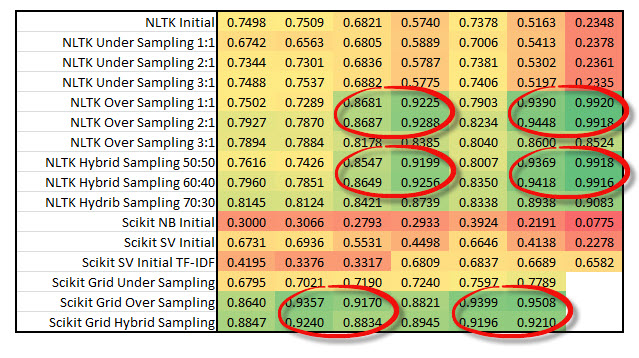
\includegraphics[width=1\textwidth]{Figures/Chapter5/best_model_01.jpg}
	\caption[Best Model - G-Performance heat map]{Heat map showing the g-performance measurement for all models}
	\label{fig:best_model_01}
\end{figure}

\subsection{Best Models}

Though the NLTK models developed using tri-grams have the best g-performance values, it was felt that it would be remiss to restrict further testing only to this model type and not to also test other model types as well. Testing will be performed in three phases. First, the top NLTK over sampling models will be analysed, followed by the top NLTK hybrid sampling model, before finally the top SciKit-Learn models are investigated.

\subsection{Initial Models}

In total 8 NLTK over sampling models were identified for further analysis. These models, listed in best g-performance order, are shown in Table \ref{tab:chapter5:top_nltk_os_models}. The first column provides a reference name for each model that will be used later for identification.

\begin{table}[h]
	\centering
	\caption[Top performing NLTK over sampling models]{Table listing the top performing NLTK over sampling models listed in order of their g-performance.}
	\label{tab:chapter5:top_nltk_os_models}
	\begin{tabular}{llrrrr}
		\toprule
		\textbf{Ref:} & \textbf{Model Type} & \textbf{Sampling} & \textbf{Stop}   & \textbf{N-Grams} & \textbf{G-Performance}  \\
		                    & \textbf{Ratio}    & \textbf{Words}  &                  &   \\
		\midrule
		1  & NLTK Over Sampling & 1:1 & Removed & Tri-grams & 0.9920  \\
		2  & NLTK Over Sampling & 2:1 & Removed & Tri-grams & 0.9918  \\
		3  & NLTK Over Sampling & 2:1 & Removed & Bi-grams  & 0.9448  \\
		4  & NLTK Over Sampling & 1:1 & Removed & Bi-grams  & 0.9390  \\
		5  & NLTK Over Sampling & 2:1 & Included & Tri-grams & 0.9288  \\
		6  & NLTK Over Sampling & 1:1 & Included & Tri-grams & 0.9225  \\
		7  & NLTK Over Sampling & 2:1 & Included & Bi-grams & 0.8687  \\
		8  & NLTK Over Sampling & 1:1 & Included & Bi-grams & 0.8681  \\
		\bottomrule
    \end{tabular}
\end{table}

Considering Table \ref{tab:chapter5:top_nltk_os_models} it is seen that training data with stop words removed produced better models than those developed using training data that included stop words. It was also seen that tri-grams have returned better results than bi-grams. However, there is not a clear sampling ratio that performs better. A Naive Bayes learner was used in all models.

In addition to the NLTK over sampling models, 8 NLTK hybrid sampling models were identified for further analysis. These models, listed in best g-performance order, are shown in Table \ref{tab:chapter5:top_nltk_hs_models}.

\begin{table}[h]
	\centering
	\caption[Top performing NLTK hybrid sampling models]{Table listing the top performing NLTK hybrid sampling models listed in order of their g-performance.}
	\label{tab:chapter5:top_nltk_hs_models}
	\begin{tabular}{llrrrr}
		\toprule
		\textbf{Ref:}  & \textbf{Model Type} & \textbf{Sampling} & \textbf{Stop}   & \textbf{N-Grams} & \textbf{G-Performance}  \\
		                    & \textbf{Ratio}    & \textbf{Words}  &                  &   \\
		\midrule
		9  & NLTK Hybrid Sampling & 50:50 & Removed & Tri-grams & 0.9918  \\
		10  & NLTK Hybrid Sampling & 60:40 & Removed & Tri-grams & 0.9916  \\
		11  & NLTK Hybrid Sampling & 60:40 & Removed & Bi-grams  & 0.9418  \\
		12  & NLTK Hybrid Sampling & 50:50 & Removed & Bi-grams  & 0.9369  \\
		13  & NLTK Hybrid Sampling & 60:40 & Included & Tri-grams & 0.9256  \\
		14  & NLTK Hybrid Sampling & 50:50 & Included & Tri-grams & 0.9199  \\
		15  & NLTK Hybrid Sampling & 60:40 & Included & Bi-grams & 0.8649  \\
		16  & NLTK Hybrid Sampling & 50:50 & Included & Bi-grams & 0.8547  \\
		\bottomrule
    \end{tabular}
\end{table}

Considering Table \ref{tab:chapter5:top_nltk_hs_models} it is seen, once again, that training data with stop words removed produced better models than those developed using training data that included stop words. It was also seen that tri-grams have returned better results than bi-grams but there is not a clear sampling ratio that performs better. A Naive Bayes learner was used in all models.

The final 8 models to consider are all Scikit-Learn models and are shown in Table \ref{tab:chapter5:top_scikit_models}

\begin{table}[h]
	\centering
	\caption[Top performing Scikit-Learn models]{Table listing the top performing Scikit-Learn models listed in order of their g-performance.}
	\label{tab:chapter5:top_scikit_models}
	\begin{tabular}{llrrrr}
		\toprule
		\textbf{Ref:}  & \textbf{Model Type} & \textbf{Samp}  & \textbf{Stop}   & \textbf{N-Grams} & \textbf{G-Perf}  \\
		                    & \textbf{Ratio} & \textbf{Words}  &                  &   \\
		\midrule
		17  & Support Vector Over Sampling & 1:1 & Included & 1, 2 & 0.9508  \\
		18  & Support Vector Over Sampling & 2:1 & Included & 1, 2, 3 & 0.9399  \\
		19  & Naive Bayes Over Sampling & 2:1 & Included & 1, 2, 3  & 0.9357  \\
		20  & Naive Bayes Hybrid Samplingng & 60:40 & Included & 1, 2, 3  & 0.9240  \\
		21  & Support Vector Hybrid Sampling & 50:50 & Removed & 1, 2, 3 & 0.9210  \\
		22  & Support Vector Hybrid Sampling & 60:40 & Included & 1, 2 & 0.9196  \\
		23  & Naive Bayes Over Sampling & 1:1 & Included & 1, 2, 3 & 0.9170  \\
		24  & Support Vector Hybrid Sampling & 70:30 & Included & 1, 2, 3 & 0.8945  \\
		\bottomrule
    \end{tabular}
\end{table}

From a quick analysis of Table \ref{tab:chapter5:top_scikit_models} the following observations can be made. It would appear that classifiers developed using the support vector learner performed slightly better than the Naive Bayes learner. It is also clear that the best model performances achieved, during training at least, was when stop words were included in the dataset and when uni-grams, bi-grams and tri-grams were utilised. There is no sampling ratio that is an obvious best performer.